\documentclass[12pt,spanish]{article}

% aprovechamiento de la p\'agina -- fill an A4 (210mm x 297mm) page
% Note: 1 inch = 25.4 mm = 72.27 pt
% 1 pt = 3.5 mm (approx)

% vertical page layout -- one inch margin top and bottom
\topmargin      -10 mm   % top margin less 1 inch
\headheight       0 mm   % height of box containing the head
\headsep          0 mm   % space between the head and the body of the page
\textheight     255 mm   % the height of text on the page
\footskip         7 mm   % distance from bottom of body to bottom of foot

% horizontal page layout -- one inch margin each side
\oddsidemargin    0 mm     % inner margin less one inch on odd pages
\evensidemargin   0 mm     % inner margin less one inch on even pages
\textwidth      159 mm     % normal width of text on page

\setlength{\parindent}{0pt}

\usepackage[doument]{ragged2e}
\usepackage{babel}
\usepackage[utf8]{inputenc}
\usepackage{amsmath,amsthm,mathtools}
\usepackage{amsfonts,amssymb,latexsym}
\usepackage{enumerate}
\usepackage{subfigure}
\usepackage{xcolor}
\usepackage{float}

\DeclarePairedDelimiter\ceil{\lceil}{\rceil}
\DeclarePairedDelimiter\floor{\lfloor}{\rfloor}

\definecolor{darkorange}{rgb}{0.94,0.4,0.0}

\usepackage{caption}

\usepackage{listings}
\lstset
{ %Formatting for code in appendix
  language=C++, % choose the language of the code
  basicstyle=\fontfamily{pcr}\selectfont\footnotesize\color{black},
  keywordstyle=\color{darkorange}\bfseries, % style for keywords
  numbers=left, % where to put the line-numbers
  numberstyle=\tiny, % the size of the fonts that are used for the line-numbers     
  backgroundcolor=\color{white},
  showspaces=false, % show spaces adding particular underscores
  showstringspaces=false, % underline spaces within strings
  showtabs=false, % show tabs within strings adding particular underscores
  tabsize=2, % sets default tabsize to 2 spaces
  captionpos=b, % sets the caption-position to bottom
  breaklines=false, % sets automatic line breaking
  breakatwhitespace=false, 
}

\begin{document}

\title{Sistemas Concurrentes y Distribuidos \\ Seminario 1: Cálculo de
  $\pi$}
\author{David Cabezas Berrido}
\date{\vspace{-5mm}}
\maketitle
\tableofcontents
\vfill
\begin{flushleft}
  {\Large Especificaciones técnicas:}
\begin{verbatim}
    Modelo: Lenovo Ideapad 700
       RAM: 8GB 
Procesador: Intel Core i7-6700HQ CPU @ 2.60GHz x 8
            (4 cores físicos, 8 lógicos)
   Gráfica: GeForce GTX 950M/PCle/SSE2
        SO: Ubuntu 18.04.1 LTS (64-bit), GNOME 3.28.2
     Disco: 1TB
\end{verbatim}
\end{flushleft}

\begin{verbatim}

\end{verbatim}
\newpage

\section{Ejercicio}
Queremos aproximar el número $\pi$ utilizando la igualdad
\[\pi = \int_0^1\frac{4}{1+x^2}dx\]
Necesitamos aproximar la integral dividiendo el intervalo $[0,1]$ en
$m$ subintervalos de igual longitud y evaluando la función en el punto
medio del intervalo para especular la altura del rectángulo. La
programación concurrente agilizará el cálculo de las áreas de los
rectángulos.

\section{Código}
He añadido las siguientes funciones para repartir los intervalos entre
las hebras y calcular la suma de las alturas, tanto de forma contigua
como entrelazada.

\begin{lstlisting}
double funcion_hebra_contigua( long i ) //Asignacion contigua
{
  long chunk = ceil(m/n);
  long top = (i+1)*chunk;
  if(i == n-1) top = m-1;
  
  double suma = 0.0;
  for(long j = i*chunk; j < top; j++) suma += f( (j+double(0.5))/m );
  
  return suma;
}


double funcion_hebra_entrelazada( long i ) //Asignacion entrelazada
{
  double suma = 0.0;
  for(long j = i; j < m-1; j+=n) suma += f( (j+double(0.5))/m );

  return suma;
}
\end{lstlisting}

En la primera función, la iteración $i$ la realiza la hebra
$\floor*{\frac{i}{n}}$. En la segunda, la realiza la hebra $i\%n$
donde $n$ es el número de hebras.

Las siguientes funciones sólo tienen que recoger la suma de cada hebra
en futuros y agruparlas.

\begin{lstlisting}
double calcular_integral_concurrente_contigua( )
{
  future<double> futuros[n];

  for(int i = 0; i < n; i++)
    futuros[i] = async(launch::async, funcion_hebra_contigua,i);

  double suma = 0.0;
  for(int i = 0; i < n; i++) suma += futuros[i].get();
  
  return suma/m;
}

double calcular_integral_concurrente_entrelazada( )
{
  future<double> futuros[n];

  for(int i = 0; i < n; i++)
    futuros[i] = async(launch::async, funcion_hebra_entrelazada,i);

  double suma = 0.0;
  for(int i = 0; i < n; i++) suma += futuros[i].get();
  
  return suma/m;
}  
\end{lstlisting}

\section{Tiempos}
He ejecutado el programa con distinto número de subintervalos y con
distinto número de hebras y he obtenido los siguientes tiempos de
ejecución.

\begin{figure}[H]
  \centering
  \subfigure[Tiempos para 8 threads]{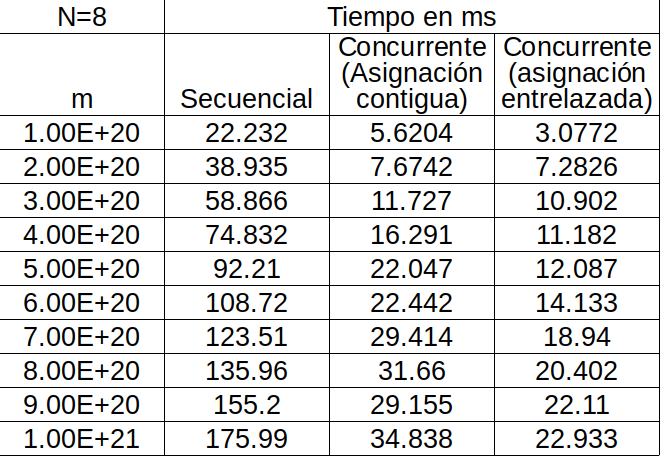
\includegraphics[width=110mm]{graficas_y_tablas/mediciones_n=8}}
  \subfigure[Tiempos para 4 threads]{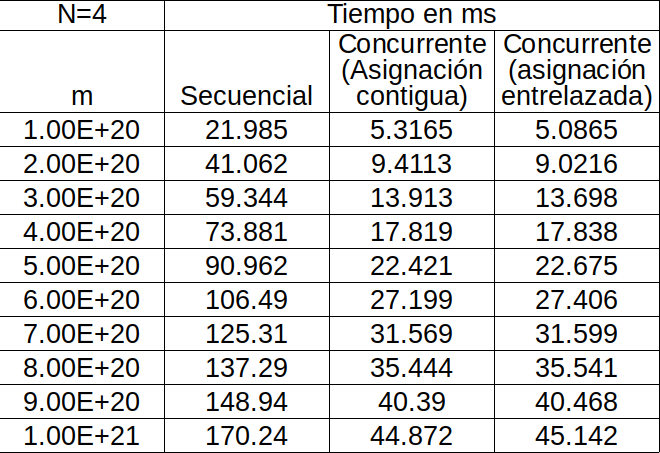
\includegraphics[width=110mm]{graficas_y_tablas/mediciones_n=4}}
\end{figure}

También he calculado la ganancia obtenida tanto en asignación
contigua como en entrelazada de los intervalos.

\begin{figure}[H]
  \centering
  \subfigure[Ganancias obtenidas]{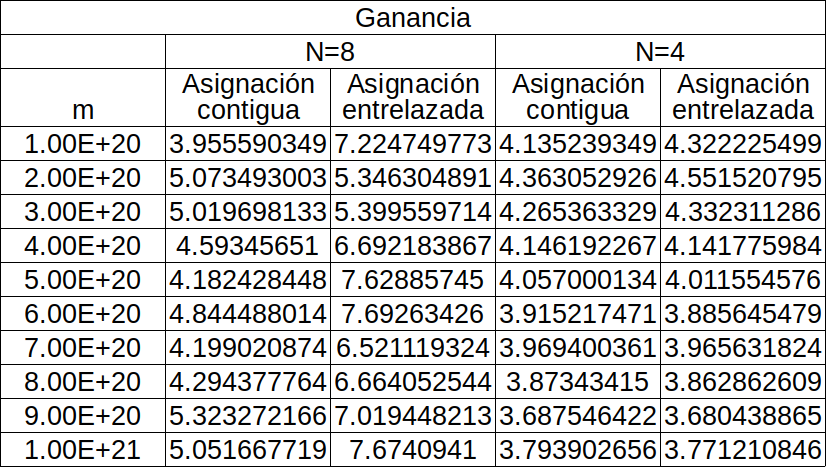
\includegraphics[width=120mm]{graficas_y_tablas/ganancia}}
\end{figure}

\section{Gráficas}
En los siguientes gráficos puede apreciarse la mejora de tiempo que
supone el uso del paralelismo, así como la ganancia obtenida.

\begin{figure}[H]
  \centering
  \subfigure[Tiempos para 8 threads]{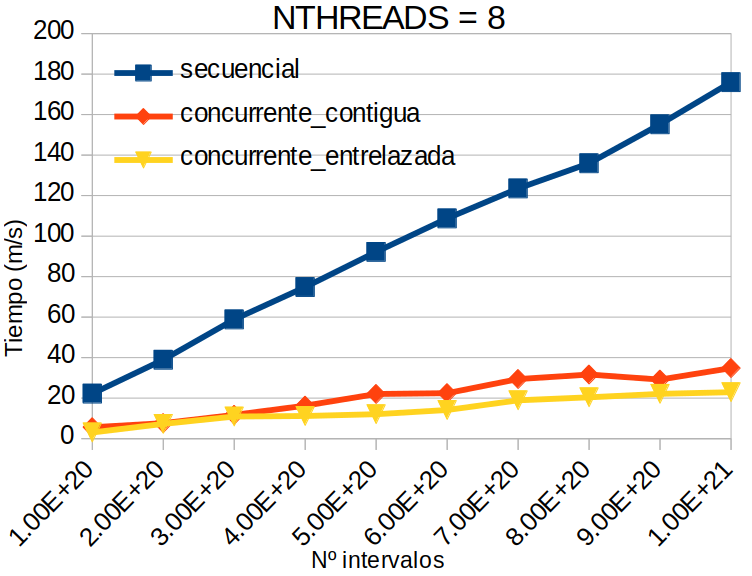
\includegraphics[width=110mm]{graficas_y_tablas/grafica_n=8}}
\end{figure}

\begin{figure}[H]
  \centering
   \subfigure[Tiempos para 4 threads]{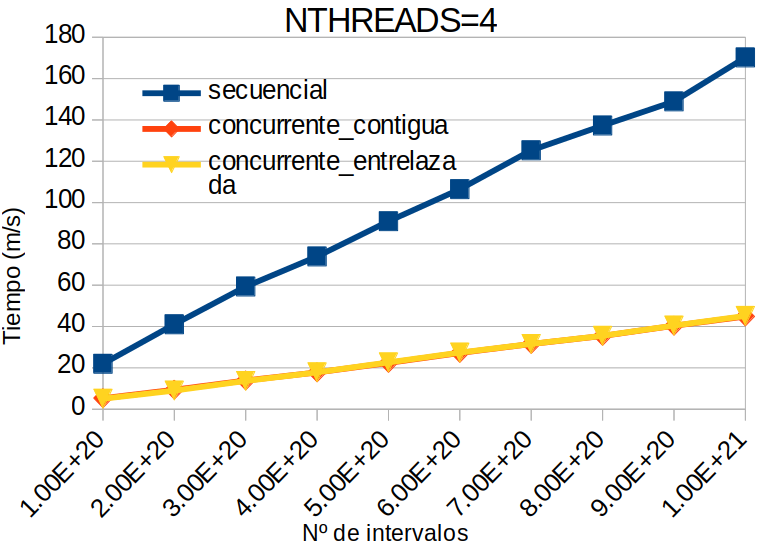
\includegraphics[width=110mm]{graficas_y_tablas/grafica_n=4}}
  \subfigure[Ganancias]{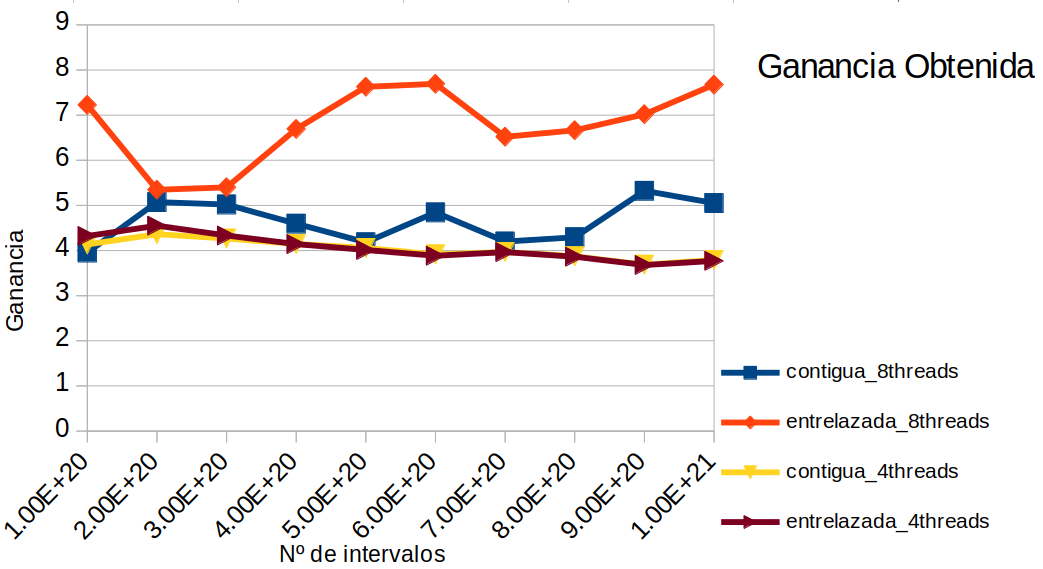
\includegraphics[width=120mm]{graficas_y_tablas/grafica_ganancia}}
\end{figure}

\section{Conclusiones}
Como era de esperar, se ha obtenido una significante mejora al
trabajar varias hebras a la vez. Se han obtenido mejores resultados
con 8 hebras que con 4 y en el caso de 8 hebras, la asignación
entrelazada ha presentado menores tiempos de ejecución.

\end{document}